% --------------------------------------------------------------
% This is all preamble stuff that you don't have to worry about.
% Head down to where it says "Start here"
% --------------------------------------------------------------
 
\documentclass[12pt]{article}
 
\usepackage[margin=1in]{geometry} 
\usepackage{amsmath,amsthm,amssymb,scrextend}
\usepackage{fancyhdr}
\usepackage{enumitem}
\usepackage{amsmath}
\usepackage{amssymb}
\usepackage{amsfonts}
\usepackage{amsbsy}
\usepackage{textcomp}
\usepackage{fancybox}
\usepackage{tikz}
\usepackage{tasks}
\pagestyle{fancy}
\usepackage[makeroom]{cancel}
\usepackage{graphicx}
\usepackage{caption}
\usepackage{mwe}
\usepackage{tikz}
\usetikzlibrary{positioning}
\usepackage{multicol}


\newcommand{\N}{\mathbb{N}}
\newcommand{\Z}{\mathbb{Z}}
\newcommand{\I}{\mathbb{I}}
\newcommand{\R}{\mathbb{R}}
\newcommand{\Q}{\mathbb{Q}}
\renewcommand{\qed}{\hfill$\blacksquare$}
\let\newproof\proof
\renewenvironment{proof}{\begin{addmargin}[1em]{0em}\begin{newproof}}{\end{newproof}\end{addmargin}\qed}
% \newcommand{\expl}[1]{\text{\hfill[#1]}$}
 
\newenvironment{theorem}[2][Theorem]{\begin{trivlist}
\item[\hskip \labelsep {\bfseries #1}\hskip \labelsep {\bfseries #2.}]}{\end{trivlist}}
\newenvironment{lemma}[2][Lemma]{\begin{trivlist}
\item[\hskip \labelsep {\bfseries #1}\hskip \labelsep {\bfseries #2.}]}{\end{trivlist}}
\newenvironment{problem}[2][Problem]{\begin{trivlist}
\item[\hskip \labelsep {\bfseries #1}\hskip \labelsep {\bfseries #2.}]}{\end{trivlist}}
\newenvironment{exercise}[2][Exercise]{\begin{trivlist}
\item[\hskip \labelsep {\bfseries #1}\hskip \labelsep {\bfseries #2.}]}{\end{trivlist}}
\newenvironment{reflection}[2][Reflection]{\begin{trivlist}
\item[\hskip \labelsep {\bfseries #1}\hskip \labelsep {\bfseries #2.}]}{\end{trivlist}}
\newenvironment{proposition}[2][Proposition]{\begin{trivlist}
\item[\hskip \labelsep {\bfseries #1}\hskip \labelsep {\bfseries #2.}]}{\end{trivlist}}
\newenvironment{corollary}[2][Corollary]{\begin{trivlist}
\item[\hskip \labelsep {\bfseries #1}\hskip \labelsep {\bfseries #2.}]}{\end{trivlist}}
 
\setlength{\parindent}{0pt}
\begin{document}
 \settasks{
	counter-format=(tsk[r]),
	label-width=4ex
}

\setcounter{section}{2}
% --------------------------------------------------------------
%                         Start here
% --------------------------------------------------------------

\lhead{Math 475}
\chead{Chapter 2}
\rhead{Meenmo K.}

\subsection{Four Basic counting Principles}
\subsubsection{Addition Principle}
{\bf Ex:} Suppose you are eating lunch at a place with 5 different sandwiches and 3 different soups. How many ways are there to order 1 meal (soup or sandwich)?
{\bf 5+3 = 8}

\end{section}

\vspace{1.5\baselineskip}
Let $S$ be a set. A \underline{partition} of $S$ is a collection of subsets $S_1,S_2,...,S_m$ such that each element of $S$ appears in {\sl exactly} one of $S_1,S_2,...,S_m$.
\begin{align}
    S &=S_1\cup S_2\cup ... \cup S_m\nonumber \\
    \phi &= S_i \cap S_j \tag{$i\neq j\quad 1\le i,\;j\le m$} \nonumber
\end{align}

\vspace{1\baselineskip}
{\bf Addition Principle}\\
Let $S_1,S_2,...,S_m$ be a partition of finite $S$. Then $$\underbrace{|S|}_{\text{\# of elements in S}} = |S_1|+|S_2|+\ldots+|S_m|$$

Jan 24 (Week 1/Thu)
\subsubsection{Multiplication Principle}
Let $S$ be a set of ordered pairs (a,b) of objects where the 1st object a comes from a set of $p$ objects and for each choice of $a$, the 2nd object $b$ has $q$ choices. Then $$|S|=p\times q$$
This comes from repeated application of the addition principle
$$|S| = \overbrace{\underbrace{q}_{\substack{\text{$q$ choices for $b$}\\ \text{given an $a$}}} + q + \ldots + q}^{p} = p\times q$$

Equivalently, if a first task has $p$ outcomes and, no matter what the outcome of the first task is, the second task has $q$ outcomes, then the number of ways of accomplishing both tasks is $p\times q$.

\vspace{1\baselineskip}
{\bf Example} Ed is picking an outfit. He has 6 distinct shirts and 4 distinct pairs of shorts. How many possible outfits (shirt and shorts) does he have? $6\times 4 = 24$

\vspace{1\baselineskip}
{\bf Example} Suppose we order a pizza with
\begin{itemize}
    \item 3 possible sizes
    \item 2 different crust styles
    \item One of 11 different toppings
\end{itemize}

How many choices of pizza do we have? $3\times 2 \times 11 = 66$

\vspace{1\baselineskip}
How many 2-digit numbers have distinct and non-zero digits? $\underline{9}\times \underline{8} = 72$

\vspace{1\baselineskip}
How many 2-digit numbers have distinct digits? $\underline{9}\times \underline{9} = 81$

\subsubsection{Subtraction Principle}
Suppose set $A$ is a subset of a larger set $U$.
$$\text{Let } \overline{A} = U \setminus A = \{x\in U: x\notin A\}$$
$$\text{Then } |A| = |U| - |\overline{A}| \text{ or } |\overline{A}| = |U|-|A|$$

{\bf Example} We are generating 6-digit passwords from the symbols 0,1,2,...,9 and a,b,c,...,z. How many passwords have a repeated digit?\\

\begin{itemize}
    \item $|U|$ := The number of set of all passwords = $36^6$
    \item $|\overline{A}|$ := The number of set of passwords with no repeated digit = $36\times 35 \times 34\times 33\times 32\times 31$
    \item $|A|$ := The number of set of passwords with a repeated digit = $|U| - |\overline{A}|$
\end{itemize}

\subsubsection{Division Principle}
Let $S$ be a finite set partitioned into $k$ parts such that each part contains the same number of objects. Then the number of parts of the partition is given by 
$$k = \frac{|S|}{\text{Common Size of Each Partition}}$$

So, the size of each partition is $\frac{|S|}{k}.$

\vspace{1.5\baselineskip}
{\bf Example} Suppose there are 740 pigeons residing in a collection of pigeonholes such that each pigeonhole contains 5 pigeons. How many pigeonholes are there?
$$k = \frac{740}{5} = 148$$

\newpage
{\bf Example} You want to make a nonempty fruit basket from 6 oranges and 9 apples. How many ways to do this?\\

{\sl Questions}
\begin{itemize}
    \item Are all apples identical? {\bf Yes}
    \item Are all oranges identical? {\bf Yes}
\end{itemize}
$$\underbrace{\underline{7}\times \underline{10}}_{\text{possible \# of oranges/apples}} - 1 =69$$

\vspace{1.5\baselineskip}
{\bf 4 Types of Counting Questions}
\begin{itemize}
    \item Arrangement and Selection
    \item Repetition and No Repetition
\end{itemize}

\subsection{Permutations}
{\bf Permutations} are arrangements \underline{without} repetition. Given a set $S$ of a distinct objects, the $r$-permutations of $S$ are the \underline{arrangements} of $r$ elements from $S$ in a distinct order.

\vspace{1.5\baselineskip}
{\bf Example} Let $S=\{a,b,c\}$. The 2-permutations of $S$ are
$$ab\qquad ba\qquad ca $$
$$ac\qquad bc\qquad cb $$

By the multiplication principle, we can readily compute $P(n,r)$, the number of $r$-permutations of a set $S$ with $n$ distinct elements.
$$P(n,r) = n\times (n-1) \times (n-2) \times \ldots \times (n-r+1)$$

\vspace{1.5\baselineskip}
\underline{Notation} 
\begin{align}
P(n,r) &= \frac{n\times (n-1) \times (n-2) \times \ldots \times (n-r+1)\times (n-r)\times (n-r-1)\times\ldots\times 2\times 1}{(n-r)\times(n-r-1)\times\ldots\times 2\times 1}\nonumber \\
&=\frac{n!}{(n-r)!} \nonumber
\end{align}

\vspace{1.5\baselineskip}
Thus $$0! = 1$$

\newpage
\subsection{Combination of Sets}
Given a set $S$ with $n$ distinct elements the $r-$combinations of $s$ are the subsets of $s$ with $r$ elements. We compute the number of $r-$combinations using the permuation formula and the division principle. The number of $r-$combinations of a set with $n$ elements is donoted $\binom{n}{r}$.
$$\binom{n}{r} = \frac{P(n,r)}{P(r,r)} = \frac{\frac{n!}{(n-r)!}}{\frac{r!}{(r-r)!}} = \frac{n!}{r!(n-r)!}$$

{\bf Circular Permutations}
Suppose we are arranging objects around a circular table (evenly space) that is free to rotate.\\

{\bf Example} 3 people (A, B, C) at a circular table. (Only 2 distinct arrangement.???) In general, for $n$ people seated at a circular table with $n$ seats. Then, there are 
$$\frac{P(n,n)}{n} = \frac{n!}{n} = (n-1)!$$ distinct ways of seating them.\\

{\bf Theorem 2.2.2} The number of $r-$circular permutations or $n$ object is given by $$\frac{P(n,r)}{r} = \frac{n!}{r(n-r)!}$$\\

{\bf Example} How many ways are there to seat to people at a circular table if 2 people will not sit next to each other?
\begin{enumerate}[label=(\roman*)]
    \item Total seating arrangement: $\frac{10!}{10}=9!$
    \item The number of cases 2 people are sitting together: $2\times \frac{9!}{9} = 2\times 8!$ \hfill (treat 2 as 1)
\end{enumerate}
Then subtract (i)-(ii).\\

{\sl Another approach}
\begin{itemize}
    \item Seat person 1: 10 ways
    \item Seat person 2: 7 ways
    \item Seat anyone else: 8! ways.
\end{itemize}
Hence $$\frac{10\times 7\times 8!}{10}$$

\newpage
% How many 2-digit numbers have distinct and non-zero digits?
% $$\underline{9}\times\underline{8} = 72$$\\

% How many 2-digit numbers have distinct digits?
% $$\underline{9}\times\underline{9}=81$$

{\bf Example} How many positive integers are factors of $3^4\times 5^2\times 11^7\times 13^8$ ?\\

Factors are $3^i\times 5^j\times 11^k\times 13^l$.
$$0\le i \le 4,\quad 0\le j \le 2,\quad 0\le k \le 7,\quad 0\le l \le 8$$

\Rightarrow 5\times 3\times 8\times 9$\\

{\bf Example} How many integers from 0 to 10,000(inclusive) have exactly 1 digit equal to 5?\\

Assume we are looking at 4-digit numbers but we allow leading zeros?\\
__________________________________\\

{\bf Example} How many ways to order the 26 letters of the alphabet so that none of a e i o u occur consecutive?\\

There are 21! ways of arranging -----. By multiplication principle, $21!\times p(22,5) = 21!\times\frac{22!}{17!}$.\\






\newpage
Feb 05 (Week3/Tue)\\

\underline{Recall}
$$\binom{n}{0}+\binom{n}{1}+...+\binom{n}{n} = 2^n \label{$n\ge 0$ where n is integer}$$

\vspace{1.5\baselineskip}
{\bf Theorem 2.3.3}(Pascal's Formula): For integers $n$ and $k$ with $n\ge 1 $ and $1\le k\le n$,

$$\binom{n}{k} = \binom{n-1}{k-1}+\binom{k-1}{k}$$

{\sl proof.} Suppose we have a set of $n$ distinct elements, and we choose $k$ of them. We know there are $\binom{n}{k}$ was to do this. On the other hand, we can do so in a fashion that pays close attention to one element of our set ( the "Golden Egg").\\

$\binom{n-1}{k}$ ways to not choose the golden egg (and $k-1$ other items). So, $\binom{n-1}{k}+\binom{n-1}{k-1}$ ways total.\\

$\Rightarrow$ These count the same thing, so $\binom{n}{k}=\binom{n-1}{k}+\binom{n-1}{k-1}$

\vspace{2\baselineskip}

$\subsection{Permutations of Multisets}$
\underline{Multisets} are sets that may contain multiple instances of the same thing. \\

{\bf Example} Suppose 5 people each buy one of 3 available computer models and there are \underline{infinitely} many computers available in each model.How many ways can these people purchase their computers? $3\times3\times3\times3\times3=3^5$\\

In this example, if we let A, B, and C denote our computer models, we are counting permutations of the multiset $$\{\infty\cdot A,\; \infty\cdot B,\; \infty\cdot C\}$$

In general, the multiset $\{n_1k_1,\;n_2k_2,...,n_rk_r\}$ indicates


$$\text{Axxx $n_i$ could be $\infty$ }
\begin{cases}
n_1 \text{ elements } k_1\\
n_2 \text{ elements } k_2\\
\vdots
\end{cases}$$

{\bf Theorem 2.4.1} Let $S$ be a multiset with objects of $r$ different types, where each element has infinite repetition number. Then the number of m-permutations is $r^m$. (Book uses different notation.)\\

{\sl proof.} Use multiplication principle.\\

{\bf Example} How many ways are there to arrange all the leeters in MISSISSIPPI?\\

{\sl Solution 1.} Treat repeated letters as distinct, to obtain 11! permutation. Now, we use the division principle and divide by $\underbrace{4!}_{4I_s}\times \underbrace{4!}_{4S_s}\times\underbrace{2!}_{2P_s}$ to compensate for repetition. This gives us $\frac{11!}{4!4!2!}$ total permutations.\\

{\sl Solution 2.} Use combinations! Choose positions for each letter.
\begin{itemize}
    \item $\binom{11}{4}$ choices for $I_s$
    \item $\binom{7}{4}$ choices for $S_s$
    \item $\binom{3}{2}$ choices for $P_s$
    \item $\binom{1}{1}$ choices for $I_s$
\end{itemize}

\vspace{2\baselineskip}
Generalizing this example, we have...\\

{\bf Theorem 2.4.2} Let $S$ be a multiset with objects of $k$ different types with finite repetition numbers $n_1,\;n_2,...,n_k,$ respectively. Let the size of $S$ be $n=n_1+n_2+...+n_k$. Then the number of permutations of $S$ equals $$\frac{n!}{n_1!n_2!\ldots n_k!}$$

\vspace{1\baselineskip}
{\bf Theorem 2.4.3} Let $n$ be a positive integer and $n_1,\;n_2,...,n_k$ positive integers such that $n_1+n_2+...+n_k=n.$ The number of ways to partition $n$ objects into $k$ labelled boxes such that 
$$\begin{cases}
\text{Box 1 contains $n_1$ items}\\
\text{Box 2 contains $n_2$ items}\\
\vdots\\
\text{Box k contains $n_k$ items is}\\
\end{cases}$$
$$\frac{n!}{n_1!n_2!\ldots n_k!}$$

\vspace{1.5\baselineskip}
If the boxes are not labelled and $n_1=n_2=...=n_k$ then the number of partitions equals $$\frac{n!}{k!n_1!n_2!...n_k!}$$

Suppose we are given an $n\times n$ chessboard and we wish to place $n$ identical rooks so that no two rooks are in attacking position. (i.e. they do not share a row or column)\\

\newpage
{\bf Example} $n=4$
%%%%tikzset
\tikzset{every picture/.style={line width=0.75pt}} %set default line width to 0.75pt        
\begin{center}



\tikzset{every picture/.style={line width=0.75pt}} %set default line width to 0.75pt        

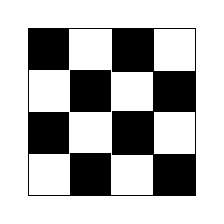
\begin{tikzpicture}[x=0.75pt,y=0.75pt,yscale=-1,xscale=1]
%uncomment if require: \path (0,300); %set diagram left start at 0, and has height of 300

%Shape: Rectangle [id:dp9985566650462854] 
\draw  [fill={rgb, 255:red, 0; green, 0; blue, 0 }  ,fill opacity=1 ] (200,20) -- (219.24,20) -- (219.24,40.07) -- (200,40.07) -- cycle ;
%Shape: Rectangle [id:dp24826412992111702] 
\draw   (200,20) -- (280.43,20) -- (280.43,100.67) -- (200,100.67) -- cycle ;
%Shape: Rectangle [id:dp41220247831592904] 
\draw  [fill={rgb, 255:red, 0; green, 0; blue, 0 }  ,fill opacity=1 ] (240.64,20.67) -- (260.43,20.67) -- (260.43,40.67) -- (240.64,40.67) -- cycle ;
%Shape: Rectangle [id:dp03987802009546293] 
\draw  [fill={rgb, 255:red, 0; green, 0; blue, 0 }  ,fill opacity=1 ] (220.4,40.2) -- (239.64,40.2) -- (239.64,60.27) -- (220.4,60.27) -- cycle ;
%Shape: Rectangle [id:dp38184662771111744] 
\draw  [fill={rgb, 255:red, 0; green, 0; blue, 0 }  ,fill opacity=1 ] (280.43,40.67) -- (260.43,40.67) -- (260.43,60.27) -- (280.43,60.27) -- cycle ;
%Shape: Rectangle [id:dp18236652736512515] 
\draw  [fill={rgb, 255:red, 0; green, 0; blue, 0 }  ,fill opacity=1 ] (200,60.4) -- (219.24,60.4) -- (219.24,80.47) -- (200,80.47) -- cycle ;
%Shape: Rectangle [id:dp38145007029970235] 
\draw  [fill={rgb, 255:red, 0; green, 0; blue, 0 }  ,fill opacity=1 ] (220.4,80.6) -- (239.64,80.6) -- (239.64,100.67) -- (220.4,100.67) -- cycle ;
%Shape: Rectangle [id:dp5477958614589156] 
\draw  [fill={rgb, 255:red, 0; green, 0; blue, 0 }  ,fill opacity=1 ] (280.43,80.67) -- (260.43,80.67) -- (260.43,100.67) -- (280.43,100.67) -- cycle ;
%Shape: Rectangle [id:dp45361950664207096] 
\draw  [fill={rgb, 255:red, 0; green, 0; blue, 0 }  ,fill opacity=1 ] (240.68,60.29) -- (260.43,60.29) -- (260.43,80.67) -- (240.68,80.67) -- cycle ;




\end{tikzpicture}

\end{center}
%%%%

There are $n!$ ways to do this:\\

Go column by column
\begin{itemize}
    \item First column has 1 rook, $n$ possible rows.
    \item Second column has 1 rook, $n-1$ possible rows.
    \item Third column has 1 rook, $n-2$ possible rows.\\
    \qquad\qquad \vdots
    \item $nth$ column has 1 rook, 1 possible rows.
\end{itemize}
Use multiplication principle.

\vspace{2\baselineskip}
Now suppose the $n$ rooks are distinct. This gives us $(n!)^2$ ways of placing the rooks in non-attacking position:
\begin{itemize}
    \item n! configurations
    \item n! rearrangements of the rooks in each configuration.
\end{itemize}

\vspace{2\baselineskip}
Feb 07 (Week3/Thu)\\
{\bf Theorem 2.4.4} The number of ways to place $n$ rooks in non-attacking position on an $n\times n$ chess board with 
$$\sum_{i=1}^k n_i = n \begin{cases}
\text{$n_1$ rooks of color 1}\\
\text{$n_2$ rooks of color 2}\\
\vdots \\
\text{$n_k$ rooks of color k}
\end{cases}$$
 
$$=\frac{(n!)^2}{n_1!n_2!\ldots n_k!}$$

\subsection{Combinations of Multisets}
{\bf Example} Suppose we order 12 doughnuts of 8 different varieties ("infinitely" many of each variety available). \\

To solve this, we think of there being 8-1=7 dividers between types of doughnuts. (We assume all doughnuts of each type are grouped together. It's ok to have zero doughnuts of a given type.)\\

So we have 19 spaces for doughuts and dividers. We choose 7 of these for the dividers.
\begin{center}
    


\tikzset{every picture/.style={line width=0.75pt}} %set default line width to 0.75pt        

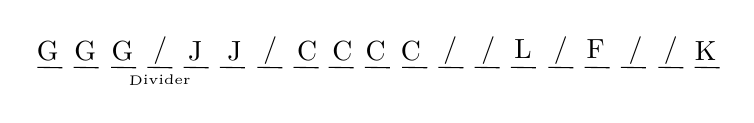
\begin{tikzpicture}[x=0.75pt,y=0.75pt,yscale=-1,xscale=1]
%uncomment if require: \path (0,300); %set diagram left start at 0, and has height of 300

%Straight Lines [id:da5669168799310167] 
\draw    (44.51,120) -- (56.56,120.2) ;


%Straight Lines [id:da746325710086311] 
\draw    (61.97,120) -- (74.02,120.2) ;


%Straight Lines [id:da8368434971403089] 
\draw    (9,120) -- (21.05,120.2) ;


%Straight Lines [id:da3154889206740792] 
\draw    (26.46,120) -- (38.51,120.2) ;


%Straight Lines [id:da009937213270028833] 
\draw    (114.94,120) -- (126.99,120.2) ;


%Straight Lines [id:da8919944526195513] 
\draw    (132.4,120) -- (144.45,120.2) ;


%Straight Lines [id:da7282216980789733] 
\draw    (79.43,120) -- (91.48,120.2) ;


%Straight Lines [id:da5366974879583333] 
\draw    (96.89,120) -- (108.94,120.2) ;


%Straight Lines [id:da8795101957139171] 
\draw    (184.79,120) -- (196.84,120.2) ;


%Straight Lines [id:da25809785222946946] 
\draw    (202.25,120) -- (214.3,120.2) ;


%Straight Lines [id:da5413197472927904] 
\draw    (149.28,120) -- (161.33,120.2) ;


%Straight Lines [id:da9152738017989683] 
\draw    (166.74,120) -- (178.79,120.2) ;


%Straight Lines [id:da7002298625284302] 
\draw    (255.22,120) -- (267.27,120.2) ;


%Straight Lines [id:da6413872229113529] 
\draw    (272.68,120) -- (284.73,120.2) ;


%Straight Lines [id:da8417124450384981] 
\draw    (219.71,120) -- (231.76,120.2) ;


%Straight Lines [id:da7997204959133808] 
\draw    (237.17,120) -- (249.22,120.2) ;


%Straight Lines [id:da9142407759921314] 
\draw    (308.19,120) -- (320.24,120.2) ;


%Straight Lines [id:da2474755672831217] 
\draw    (325.65,120) -- (337.7,120.2) ;


%Straight Lines [id:da7713017538867706] 
\draw    (290.14,120) -- (302.19,120.2) ;



% Text Node
\draw (14,112) node  [align=left] {G};
% Text Node
\draw (32,112) node  [align=left] {G};
% Text Node
\draw (50,112) node  [align=left] {G};
% Text Node
\draw (66,112) node  [align=left] { \ /};
% Text Node
\draw (68,126) node [rotate=-359.13,xslant=0.06] [align=left] {{\tiny  Divider}};
% Text Node
\draw (85,112) node  [align=left] {J};
% Text Node
\draw (104,112) node  [align=left] {J};
% Text Node
\draw (119,112) node  [align=left] { \ /};
% Text Node
\draw (139,112) node  [align=left] {C};
% Text Node
\draw (156,112) node  [align=left] {C};
% Text Node
\draw (172,112) node  [align=left] {C};
% Text Node
\draw (189,112) node  [align=left] {C};
% Text Node
\draw (208,112) node  [align=left] { /};
% Text Node
\draw (259,112) node  [align=left] { \ /};
% Text Node
\draw (224,112) node  [align=left] { \ /};
% Text Node
\draw (295,112) node  [align=left] { \ /};
% Text Node
\draw (312,112) node  [align=left] { \ /};
% Text Node
\draw (331,112) node  [align=left] {K};
% Text Node
\draw (278,111) node  [align=left] {F};
% Text Node
\draw (243,111) node  [align=left] {L};


\end{tikzpicture}

\end{center}
So the number of doughnut orders is $\binom{12+8-1}{8-1}=\binom{19}{7}$.\\

{\sl Recall}: $\binom{19}{7} = \binom{19}{12} \leftarrow$ ways to position the doughnuts themselves.\\

{\bf Theorem 2.5.1} Let $S$ be a multiset with objects of $k$ different types, each with infinite repetition number. Then the number of $r$-combinations of $S$ equals $$\binom{r+k-1}{r}=\binom{r+k-1}{k-1}$$\\

{\sl Proof Idea} This is just like the doughnut example with $r$ doughnuts and $k$ varieties.\\

Note that our doughnut example gave us solutions to 
%%%%%%%%%%%%%%%%%%%%%%%%%%%%%%%%%%%%%%%%%%%%%
\begin{align*}
    \sum_{i=1}^8 n_i = 12 \label{\text{where each } n_i \text{ is non-negative integer}}
\end{align*}
%%%%%%%%%%%%%%%%%%%%%%%%%%%%%%%%%%%%%%%%%%%%%

What if $n_2\ge 2$? Then let $n_2'=n_2-2$. So $n_2'\ge 0$. Look at $n_1+n_2'+n_3+\ldots+n_8=10$\\

{\bf Example} What is the number of non-decreasing sequences of length $r$ taken from the numbers $1,2,...,k$?\\

We are choosing $r$ things from the multiset $\{\infty\cdot 1,\;\infty\cdot2,\ldots,\; \infty\cdotk\}$. So we have $$\binom{r+k-1}{r}=\binom{r+k-1}{k-1} \text{ choices.}$$

{\bf Example} the number of ways to distribute 9 identical apples to 3 kids $\binom{9+3-1}{3-1}$ (9 apples, 3 "varieties" based on which kid gets each.) 
\begin{center}
   


\tikzset{every picture/.style={line width=0.75pt}} %set default line width to 0.75pt        

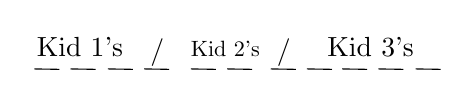
\begin{tikzpicture}[x=0.75pt,y=0.75pt,yscale=-1,xscale=1]
%uncomment if require: \path (0,300); %set diagram left start at 0, and has height of 300

%Straight Lines [id:da5630468125749615] 
\draw    (64.51,179) -- (76.56,179.2) ;


%Straight Lines [id:da9164470523542558] 
\draw    (81.97,179) -- (94.02,179.2) ;


%Straight Lines [id:da5985754595668842] 
\draw    (29,179) -- (41.05,179.2) ;


%Straight Lines [id:da09636442877505225] 
\draw    (46.46,179) -- (58.51,179.2) ;


%Straight Lines [id:da29278478556962484] 
\draw    (142.94,179) -- (154.99,179.2) ;


%Straight Lines [id:da9573040787535034] 
\draw    (160.4,179) -- (172.45,179.2) ;


%Straight Lines [id:da10712452445077036] 
\draw    (104.43,179) -- (116.48,179.2) ;


%Straight Lines [id:da031576740745527854] 
\draw    (121.89,179) -- (133.94,179.2) ;


%Straight Lines [id:da13295652784395418] 
\draw    (212.79,179) -- (224.84,179.2) ;


%Straight Lines [id:da7038175080037512] 
\draw    (177.28,179) -- (189.33,179.2) ;


%Straight Lines [id:da7230546132452242] 
\draw    (194.74,179) -- (206.79,179.2) ;



% Text Node
\draw (86,171) node  [align=left] { \ /};
% Text Node
\draw (147,171) node  [align=left] { \ /};
% Text Node
\draw (51.05,168.2) node  [align=left] {Kid 1's};
% Text Node
\draw (121.05,169.2) node [scale=0.8] [align=left] {Kid 2's};
% Text Node
\draw (191.05,168.2) node  [align=left] {Kid 3's};


\end{tikzpicture}

\end{center}
\subsection{Probability}
{\sl Idea} There is an experiment $\zeta$ with a set of outcomes sample space $S$. An event $E$ is a subset of $S$. We will assume all outcomes are equally likely.\\

{\bf Example} Suppose our experiment is rolling two [6-sided] dice (one blue, one red).
\begin{align}
    S&=\{(1,1),(2,1),(3,1),(4,1),(5,1),(6,1)\nonumber \\
    &\qquad (1,2),(2,2),(3,2),(4,2),(5,2),{\bf (6,2)}\nonumber \\
    &\qquad (1,3),(2,3),(3,3),(4,3),{\bf (5,3)},(6,3)\nonumber \\
    &\qquad (1,4),(2,4),(3,4),{\bf (4,4)},(5,4),(6,4)\nonumber \\
    &\qquad (1,5),(2,5),{\bf (3,5)},(4,5),(5,5),(6,5)\nonumber \\
    &\qquad (1,6),{\bf (2,6)},(3,6),(4,6),(5,6),(6,6)\nonumber\}
\end{align}

Let $E$ be the event that the dice roll adds to 8.
$$E=\{(2,6),(3,5),(4,4),(5,3),(6,2)\}$$
\begin{itemize}
    \item $S$ has 36 elements
    \item $E$ has 5 elements
\end{itemize}

In this case, we say that the probability of event $E$ occurring is $\frac{5}{36}$. In generally, the \underline{probability} of event of event $E$ is $$P(E) = \frac{|E|}{|S|}.$$\\
Note that $0\le P(E)\le 1$.\\

{\sl Cool Trick:} Sometimes figuring out the probability that something \underline{will not} happen and subtracting this from 1 is easier.\\

In other words, $$P(\overline{E}) = 1-P(E).$$\\

{\bf Example} To compute the probability that 2 people in a group share a birthday, compute the probability that they do not share a birthday. Given $n$ people, there are $365^n$ birthday possibilities (Ignoring Feb 29).\\

There are $P(365,n)$ ways they can have distinct birthdays (Assuming $n\le 365$). So, the probability of an unshared birthday is $$\frac{\frac{365!}{(365-n)!}}{365^n}$$. The probability of a shared birthday is $$1-\frac{\frac{365!}{(365-n!)}}{365^n}$$






\end{document}